\chapter{Änderungen durch neue Antriebe, Annahmen und Methodik}
\label{ch:Änderungen durch neue Antriebe, Annahmen und Methodik}

Konzepte mit neuen Antrieben befinden sich in der Entwicklung.
Daher sollte in Erwägung gezogen werden, wie zukünftige Flughäfen 
gestaltet werden und welche Ausstattung für 
die Flugzeugabfertigung zum Einsatz kommt.
Wasserstoff-Flugzeuge werden erst ab dem Jahr 2035 auf den Markt kommen, 
wobei die batteriebetriebenen Flugzeuge schon in den nächsten Jahren erwartet werden.
Der Wechsel zu nachhaltigen Antrieben kann zu deutlichen Änderungen 
in der Infrastruktur und Abläufen am Vorfeld führen, 
welche in diesem Kapitel beschrieben werden.
Außerdem werden auf Grundlage der unterschiedlichen Quellen und 
vernünftigen Behauptungen eine Reihe von Annahmen für diese Arbeit getroffen.
%Dieser Teil der Arbeit beschäftigt sich mit der vorhandenen Infrastruktur-Optionen. %und im Fall des Wasserstoffs Lieferketten.
%
%Wenn die Infrastruktur auf den Regionalflughäfen gemacht wird, 
%macht es nicht so ein Ausmaß wie auf größeren Flughäfen, wo viele Abfertigungsplätze umgerüstet werden müssen.

\section{Änderungen an der Betrieb/Infrastruktur und dazugehörige Kosten von alternativen Antrieben}
\label{s:Änderungen an der Abfertigung und dazugehörige Kosten von alternativen Antrieben}

Infrastrukturkosten sind von der Größe des Flughafens abhängig. 
Größere Flughäfen können mehr Flugzeuge als Regionalflughäfen abfertigen, 
was dazu führt, dass mehr Abfertigungsplätze umgerüstet und versorgt, 
sowie mehr Arbeitskräfte geschult werden müssen. 
In diesem Teil wird näher auf die Änderungen der Infrastruktur durch 
die Einführung von neuen Antrieben eingegangen und bestimmte Szenarien ausgewählt.

\subsection{SAF am Flughafen}
SAF ist aufgrund vorhandener Emissionen zwar nicht die beste langfristige Lösung, 
aufgrund der Notwendigkeit weiterer Entwicklungen der alternativen nachhaltigen 
Antriebe stellt es aber eine gute Option dar. 
In naher Zukunft werden vor allem die großen Flugzeuge nicht mit Batterieantrieb entwickelt, 
deswegen kann SAF für Langstreckenflüge genutzt werden \cite{dalmia2022powering}.
Diese Arbeit wird sich auf das reine SAF ohne Beimischung beschränken, 
da nur so das gesetzte Ziel bis zum Jahr 2050 erreicht werden kann.

SAF benötigt keine Infrastrukturänderung und darf in bestehenden Systemen 
und Flugzeugen genutzt werden \cite{dalmia2022powering}.
Dadurch, dass SAF zu herkömmlichen Treibstoffen beigemischt wird, 
wird zurzeit ein zusätzlicher Tank für den gemischten Kraftstoff benötigt. 
Bis heute ist der Transport von SAF durch eine Pipeline nicht zugelassen (Quelle?). %%%%%%%%%%%%%%QUELLE
Nach intensiver Recherche wurde jedoch keine Information gefunden, 
die besagt, dass es verboten sein wird, reines SAF nicht als Drop-In zu nutzen.
Aus diesem Grund gilt für die Arbeit, dass die Lieferung von SAF mit bestehenden Pipelines 
zertifiziert und genau wie bei der Betankung mit herkömmlichen Treibstoffen zugelassen wird.

\subsection{Batterieantrieb am Flughafen}
Batteriebetriebene Flugzeuge brauchen größere Veränderung am 
Flughafen als bei der Nutzung von SAF.
Bis zum Jahr 2050 sind die Batterieantriebe auf kleinere Flugzeuge 
und damit auf Kurz- und Regionalverkehr beschränkt. 

In der Literatur werden zwei Batterie-Lademöglichkeiten diskutiert, 
einerseits das Wechseln der Batterien (Swap-Methode), 
bei welcher diese aus dem Flugzeug herausgenommen und an einer Ladestation geladen werden, 
andererseits die Batterien des Flugzeugs per Ladekabel aufzuladen (Plug-In), 
ähnlich wie bei etablierten E-Autos.
Zudem ist ein modulares System möglich, bei welchem beide Ansätze genutzt werden \cite{salucci2020optimal}.
%
Bei diesem Antrieb muss beachtet werden, 
welche Lebensdauer eine Batterie hat und wie die Batterien geladen werden. 
Je länger die Ladung dauert, desto mehr Kosten werden auf dem Boden verursacht. 
Nichtsdestotrotz kann eine schnelle Ladung zur Reduktion der Lebensdauer einer Batterie führen (Quelle!!).

Die Ladeleistung ist für die Dauer der Ladung verantwortlich. 
Durch schnellere Ladungen wird die Lebensdauer der Batterien reduziert,
was verursacht, dass die Batterien schneller ausgetauscht werden 
müssen, wodurch mehr Kosten entstehen.
%Das langsame Laden ist für Fluggesellschaften nicht rentabel, 
%da wenn Flugzeug auf dem Boden steht, verdienen die Fluggesellschaften kein Geld.

%
Die \textit{Plug-In} Methode benötigt ein schnelles Laden, 
damit Flugzeuge weniger Zeit auf Boden verbringen müssen.
Jedoch ist ein Anstieg der Turnaround-Zeiten aufgrund der 
nicht existierenden Schnellladung vorstellbar \cite{avogadro2024demystifying}. %es ist anwendbar, existiert einfach noch nocht

Bei der \textit{Swap-Methode} kann der Aus- und Einbau der Batterie aus 
und in das Flugzeug lange dauern \cite{dalmia2022powering}. 
Guo et al. \cite{guo2020aviation} ist zu dem Schluss gekommen, 
dass Batteriewechsel effizienter und ökonomischer sind, 
wenn die batteriebetriebenen Flugzeuge nur einen kleinen Teil (unter 10 \%) der Flotte darstellen, 
in anderen Fällen lohnt sich eine Plug-In-Ladung. 
Für Batteriewechsel müssen auch Transport und Hebegeräte gestellt werden, 
um die Batterien bewegen zu können \cite{reimers2018introduction}.
%Jedoch können mit dem Batteriewechsel die Abfertigungszeiten reduziert werden (Quelle), 
%was an einem großen Flughafen von Bedeutung ist. 
Besonders an einem großen Flughafen kann die Dauer der Abfertigung von Bedeutung sein.
Der Batteriewechsel bietet gleichmäßigere Deckung der Nachfrage \cite{guo2020aviation} 
und ist kompatibler mit der Flugplanung \cite{salucci2020optimal}, 
da der Austausch einer Batterie schneller ist, als die Dauer einer Plug-In Ladung. 
Jedoch werden mehrere Batterien benötigt, 
die zudem ordnungsgemäß und sicher gelagert werden müssen \cite{salucci2020optimal}.
Außerdem ermöglicht die Swap-Methode langsameres Laden und macht 
das Laden mit geringerer Leistung möglich \cite{avogadro2024demystifying}.
%Aus diesen Gründen werden in den nächsten Teilen 
%der Arbeit die Kosten für diese Option ausgewertet. 

Würde der Austausch der Batterien parallel zu anderen Prozessen, 
wie bspw. Deboarding stattfinden, könnte eine kürzere Turnaround-Zeit im 
Vergleich zu konventionellen Flugzeugen erreicht werden \cite{schmidt2016challenges}.

\textit{Annahmen für die BA-Analyse}\\
%
Für die weitere Betrachtung wurde sich für die Swap-Methode entschieden. 
Zudem wird angenommen, dass die Batterien für Flugzeuge zur Flughafen-Infrastruktur gehören.
Das bedeutet, dass diese Anschaffungskosten für den Flughafen anfallen 
und diese in Form von Leasinggebühren für Fluggesellschaften weitergegeben werden.

Für die Ladevorgänge wird Strom benötigt. 
Die Strompreise und die verfügbare Leistung hängen normalerweise 
von den Tag- und Nachtzeiten ab \cite{salucci2020optimal}. 
Aus praktischen Gründen wird eine konstante Spitzenleistung des Batterieladesystems von 250 kW wird angenommen. 
Bei einer Batteriekapazität von 900 kWh, würde die Ladung bei einer solchen Leistung, 
ohne Beachtung der Verluste, 3,6 Stunden dauern.

%%%%%%%
%Außerdem ist ein Anstieg der Turnaround-Zeiten aufgrund 
%auch deshalb nicht möglichen Schnellladens vorstellbar \cite{avogadro2024demystifying}.
%Für die Ladung den batteriegetriebene-Flugzeugen Infrastruktur:
%Infrastrukturmodell nach Guo et al. "Die EA-Aufladung wird teilweise von einer flughafenbasierten Solar-PV-Anlage geliefert.
%Jährliche Betriebskosten (OPEX)= Strombezugskosten aus dem Netz in der Sommer und Wintersaison (typische Tage) basierend auf der Nachfrage. \cite{guo2020aviation}

\subsection{Wasserstoffantrieb am Flughafen}
Logistik ist ein wichtiger Teil der Produktionskette. 
Die Nutzung von Wasserstoff am Flughafen erfordert einen Austausch der 
Betankungsanlagen und Anschaffung neuer Lieferketten, 
um Wasserstoff als Treibstoff nutzen zu können. 
Diese Investitionskosten werden die Flughafenbetreiber belasten.
\subsubsection{Transport}
Die Lieferketten und die Produktion des Wasserstoffs spielen 
eine große Rolle in der vorhandenen Literatur.
Der Transport ist durch Pipelines im gasförmigen Zustand, 
durch LKW und Züge sowohl im gasförmigen, als auch im flüssigen Zustand möglich. 
Kapitel \ref{ss:Wasserstoff-Antrieb} stellte die möglichen physischen Formen 
von Wasserstoff fest und legte am Ende dar, 
dass flüssiger im Vergleich zum gasförmigen 
Wasserstoff für den Transport vorteilhafter ist. 
Außerdem kann er auch in einer chemischen Verbindung, 
wie Ammoniak und Methanol, gebunden und somit transportiert werden.
%
%
%Wasserstoff kann hochentzündlich sein \cite{dalmia2022powering}. %(prüfen ob entzündlicher als Kerosin)
%
% 
Die Effizienz der Produktion- und Lieferkosten ist geografisch determiniert. 
Die Lieferoptionen sind nach geografischer Position des Flughafens zu wählen. 
Für die Flughäfen, die nahe einer Wasserstoff-Pipeline liegen, ist es sinnvoller
hiermit den Wasserstoff zu transportieren, als ihn bspw. mit einem LKW liefern zu lassen.
%
Für Distanzen im europäischen Raum sind Wasserstoff-Pipelines
günstiger als der Transport mit chemischen Verbindungen, 
welcher bei längeren Distanzen in Betracht gezogen wird \cite{undertaking2022strategic}. 
Bei der Umwandlung von Erdgas- in Wasserstoffleitungen können Kosten gespart werden \cite{undertaking2022strategic}. 
Es muss keine neue Infrastruktur gebaut, nur eine Umrüstung der 
Leitungen für den Transport von Wasserstoff durchgeführt werden.

Der Transfer von \ce{LH2} mit vakuumisolierten Pipelines beschränkt sich auf kurze Distanzen
aufgrund der proportionalen Skalierung der Verluste zur Leitungslänge \cite{colpan2022fuel}.

Colpan et al.\cite{colpan2022fuel} ist der Meinung, 
das für den Fall das große Mengen an Wasserstoff benötigt werden, 
wäre die Lieferung weder per LKW, noch per Pipeline sinnvoll. 
%
Dennoch kann lt. Schenke et al. \cite{schenke2024lh2} die Lieferung des flüssigen Wasserstoffs 
mit einem LKW bei einer hohen Anzahl an Flügen kostengünstiger als andere Lieferalternativen sein.
Allerdings erfordert der Transport von \ce{LH2} speziell konstruierte Tanks \cite{mulder2019outlook}.

%Die Lieferung von gasförmigem Wasserstoff mit niedrigem Druck 
%ist im Straßenverkehr bis jetzt nur für ungenügende Mengen möglich \cite{undertaking2022strategic}
%
%Obwohl hohe Kapitalkosten für Pipeline-Anlagen zu erwarten sind, 
%werden die Betriebskosten niedriger sein \cite{mulder2019outlook}. 
%Also lohnt es sich bei größerem Umfang Pipelines zu verwenden, 
%andernfalls kommt ein Transport per LKW in Frage. \cite{mulder2019outlook}.

\textit{Speicherung}\\
Gasförmiger Wasserstoff kann unterirdisch in Salzkavernen 
und in erschöpften Gasfeldern gespeichert werden \cite{undertaking2022strategic}, 
diese müssen sich in unmittelbarer Nähe des Flughafens befinden. 
Da diese Gegebenheit je nach Flughafenstandort variiert, 
wird diese Speicheroption nicht weiter behandelt.
Außerdem kann für die Lagerung ein oberirdischer Druckzylinder eingesetzt werden, 
in welchem Wasserstoff in flüssiger oder in fester Form wie Metallhybriden gespeichert wird.
Aufgrund der tiefen Temperaturen müssen diese Zylinder oder Tanks gut isoliert und kryogen sein \cite{undertaking2022strategic}.
Andernfalls verdampft flüssiger Wasserstoff bei der Lagerung, 
was zu Verlusten führt \cite{undertaking2022strategic}. 
Die Verdampfung wird mit größeren Lagern kleiner \cite{colpan2022fuel}.

Dennoch findet der größte Teil der Verdampfung aufgrund 
der Transferphase statt \cite{undertaking2022strategic}.
%Wasserstoff kann in Hochdrucktanks und Salzkavernen gelagert werden \cite{mulder2019outlook}
Somit muss der Weg zwischen der Betankung und dem Speicher kurz sein, 
damit Verdampfungsverluste minimiert werden \cite{colpan2022fuel}

%
Eine weitere mögliche Betankungsoption ist der Austausch des Flugzeugtanks in Form von Kapseln. 
Dabei werden die leeren Kapseln an die Wasserstoffproduktionsstelle zurückgegeben, 
bei welcher diese wieder nachgefüllt werden \cite{colpan2022fuel}. 
Diese Möglichkeit kann vor allem für kleinere Flughäfen eine Alternative darstellen, 
da kein Wasserstoffspeicher oder sonstige Anlagen bereitgestellt werden müssen.
Für längeres Parken von Luftfahrzeugen am Flughafen werden gekühlte Tanks eine sichere Verbindung 
mit der Wasserstoffinfrastruktur benötigen \cite{colpan2022fuel}. %weiß nicht
%"current FCEV system costs higher than 200 €/kW for passenger cars but need 
%to fall below 50 €/kW for mass market. " \cite{undertaking2022strategic}
%
%
%neue terminals: In dem Fall, falls die Flugzeuge länger als übliche Modelle werden, die Sicherheitssperzone für die Betankung 20 Meter betragen kann \cite{gu2023hydrogen}
%
%
%"Flüssiger Wasserstoff muss jedoch bei Minusgraden gelagert werden, was eine Verbesserung der Speichertechnologien sowohl im Flugzeug selbst als auch auf Flughäfen erfordert."
%Wasserstoff kann entweder als Brennstoff für Verbrennung genutzt werden oder als Wasserbrennstoffzelle für die elektrischen Flugzeuge. \cite{dalmia2022powering}

In dem Unterkapitel \ref{ss:Wasserstoff-Antrieb} wurde angeführt, 
dass die Produktion des Wasserstoffs viel Platz und Energie benötigt und hohe Kosten verursacht. 
Eine Produktion und Verflüssigung des Wasserstoffs am Flughafen würde 
ebenfalls hohe zusätzliche Infrastrukturkosten verursachen \cite{dalmia2022powering}.
Deswegen wäre für die Flughäfen eine bessere Alternative, den Wasserstoff extern einzukaufen 
und per LKW oder Pipelines zum Flughafen liefern zu lassen \cite{gu2023hydrogen}.
Aufgrund aufwendiger und kostenintensiver Infrastrukturprozesse für die Produktion 
und Verflüssigung von Wasserstoff werden wahrscheinlich Flughäfen, 
besonders kleinere, anfangs auf die \glqq On-Site \grqq{} Produktion verzichten.

%In der Arbeit Dalmia et al. \cite{dalmia2022powering} wird die Produktion am Flughafen diskutiert. 
%Dazu wird einen Elektrolyseur für Erzeugung des gasförmigen Wasserstoffs, einen Kompressor und einen Tankwagen oder
%eine Pipeline mit modularem Tanksystem für Betankung der Flugzeuge benötigt. 
%Modulares Tanksystem kann in bestehenden Flugzeugen eingesetzt werden
%und wird als wie Fracht in das Flugzeug geladen. %(nochmal nachlesen)
%
%Für die Wasserstofferzeugung wäre die ideale Methode der Elektrolyse, die mit Strom betrieben würde, der vor Ort aus 
%erneuerbaren Ressourcen erzeugt würde, wie z. B. Solarenergie aus nicht reflektierenden Paneelen (um eine Blendung der 
%Solarmodule für Piloten zu vermeiden). Das Wasser, das für den Prozess verwendet wird, wird aus nahe gelegenen 
%Wasserquellen stammen, einschließlich Süßwasserflüssen und Seen. Diese Wasserstoffproduktion wird vor Ort an Flughäfen 
%stattfinden. Die benötigte Infrastruktur umfasst einen Elektrolyseur, einen Kompressor und einen Tankwagen. 
%Der Elektrolyseur wird gasförmigen Wasserstoff erzeugen. Der Kompressor erhöht dann den Druck des Wasserstoffs, 
%indem er sein Volumen für die Speicherung reduziert, und der Tankwagen transportiert den komprimierten Wasserstoff 
%zum Elektroflugzeug. Eine weitere Option für den Transport wäre die Installation einer landseitigen bis luftseitigen Pipeline,
% die den komprimierten gasförmigen Wasserstoff in einem modularen Tanksystem transportiert. Dieses System ermöglicht 
% die Nachrüstung von bereits im Einsatz befindlichen Flugzeugen. Die Wasserstofftanks würden ähnlich wie Fracht 
% in ein Flugzeug geladen, festgeschnallt und sicher mit dem Flugzeug verbunden. Wenn das Ziel erreicht ist, 
% wird der leere Tank durch einen neuen Tank ersetzt, der dann zurückgeschickt wird, um in der Wasserstoffproduktionsanlage 
% am Flughafen wieder aufgefüllt zu werden. Dieses System ermöglicht den Einsatz von Wasserstoff in allen Bereichen des Fluges,
% wodurch die Effizienz maximiert, das Gesamtgewicht reduziert und die Nutzlast und Reichweite verbessert werden.²³\cite{dalmia2022powering}
%
%Gerade wird Wasserstoff durch die Pipelines transportiert \cite{mulder2019outlook}. ist es so?
%Der Transport ist durch Pipelines im gasförmigen Zustand, LKW und Zügen sowohl im gasförmigen,
% als auch im flüssigen Zustand möglich. 
% Transport von LH2 erfordert speziell konstruierte Tanks \cite{mulder2019outlook}

%"Eine Kryopumpe 
%bringt den Wasserstoff auf den benötigten Druck von 1000 bar. " ?file:///C:/Users/henri/Downloads/765438.pdf

\textit{Annahmen für die Analyse}\\
Die Gesamtinvestitionen sind von der Wahl der Produktion, Speicherung, 
Lieferketten als auch der Betankungsentscheidung abhängig.
Da derzeit nicht einsehbar ist, welche Technologie umgesetzt wird, 
fokussiert sich die Arbeit auf einen bestimmten Versorgungsweg.

Die externe Produktion ist am Anfang sinnvoll \cite{colpan2022fuel}. 
Aus diesem Grund wurde angenommen, dass die Produktion des Wasserstoffs
und die Verflüssigung nicht am Flughafen stattfinden, 
der Wasserstoff stattdessen eingekauft und per LKW zum Flughafen transportiert wird.
Am Flughafen wird der Wasserstoff in kryogenen Tanks gespeichert 
und durch Betankungswägen werden die Flugzeuge mit Kraftstoff befüllt.
%
Die Lieferkosten für flüssigen Wasserstoff \ce{LH2} werden nicht explizit ausgerechnet,
da diese schon in den Betriebskosten von wasserstoffbetriebenen Flugzeugen eingeschlossen sind.
%kommt noch was dazu %%%%%%%%wird noch geändert
Die Abbildung \ref{supply_wasserstoff} stellt eine Variante von 
Produktions- und Lieferketten für flüssigen Wasserstoff dar.
Dabei werden außerhalb des Flughafens erneuerbare Energiequellen 
für die Produktion des Wasserstoffs durch Elektrolyse genutzt.
Im Weiteren wird gasförmiger Wasserstoff verflüssigt und 
in einem LKW zum Flughafen \glqq farm tank \grqq{} geliefert, 
wo er dann mit Hilfe einer Kryopumpe in einen Speicher geladen wird.
\begin{figure}[h]
	\centering
	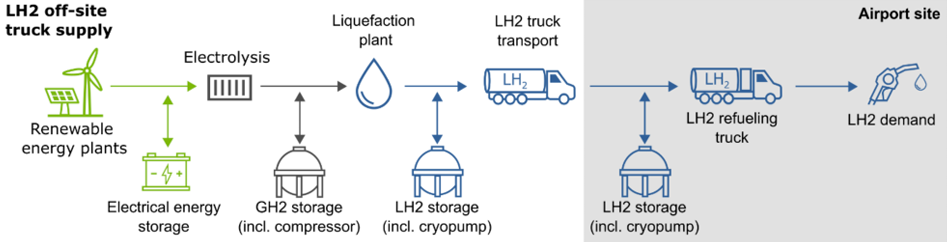
\includegraphics[width=0.9\linewidth]{Bilder/Supply_hydrogen.png}
	\caption[Lieferkette von flüssigem Wasserstoff mit externer Herstellung und interner Lagerung bzw. die Betankung]{Lieferkette von flüssigem Wasserstoff mit externer Herstellung und interne Lagerung bzw. die Betankung \cite{schenke2024lh2}}
	\label{supply_wasserstoff}
\end{figure}

%Zusätzlich wird davon ausgegangen, dass der Sicherheitsradius bei der Wasserstoffbetankung nicht erweitert wird.
